\documentclass[12pt]{article}
\usepackage[margin=2.5cm]{geometry}
\usepackage{enumerate}
\usepackage{amsfonts}
\usepackage{amsmath}
\usepackage{fancyhdr}
\usepackage{amsmath}
\usepackage{amssymb}
\usepackage{amsthm}
\usepackage{mdframed}
\usepackage{graphicx}
\usepackage{subcaption}
\usepackage{adjustbox}
\usepackage{listings}
\usepackage{xcolor}
\usepackage{booktabs}
\usepackage[utf]{kotex}
\usepackage{hyperref}
\usepackage{accents}

\definecolor{codegreen}{rgb}{0,0.6,0}
\definecolor{codegray}{rgb}{0.5,0.5,0.5}
\definecolor{codepurple}{rgb}{0.58,0,0.82}
\definecolor{backcolour}{rgb}{0.95,0.95,0.92}

\lstdefinestyle{mystyle}{
    backgroundcolor=\color{backcolour},
    commentstyle=\color{codegreen},
    keywordstyle=\color{magenta},
    numberstyle=\tiny\color{codegray},
    stringstyle=\color{codepurple},
    basicstyle=\ttfamily\footnotesize,
    breakatwhitespace=false,
    breaklines=true,
    captionpos=b,
    keepspaces=true,
    numbers=left,
    numbersep=5pt,
    showspaces=false,
    showstringspaces=false,
    showtabs=false,
    tabsize=1
}

\lstset{style=mystyle}

\pagestyle{fancy}
\renewcommand{\headrulewidth}{0.4pt}
\lhead{CSC 343}
\rhead{Worksheet 4 Solution}

\begin{document}
\title{CSC343 Worksheet 4 Solution}
\maketitle

\bigskip
\begin{enumerate}[1.]
    \item
    \begin{enumerate}[a)]
        \item $[(1,0,1),(5,4,9),(1,0,1),(6,4,16),(7,9,16)]$
        \item $[(1,0),(3,3),(3,4),(4,3),(1,1),(4,3)]$
        \item $[(0,1),(0,1),(2,3),(2,4),(3,4)]$

        \bigskip

        \underline{\textbf{Notes:}}

        \bigskip

        \begin{itemize}
            \item $\tau_L(R)$ sorts tuples in order indicated by $L$.
            \begin{itemize}
                \item e.g.

                \bigskip

                $\tau_{C,B}(R)$ in $R(A,B,C)$ orders the tuples of $R$ by their
                values of $C$, and tuples with the same $C$-value are ordered by their
                $B$ value.
            \end{itemize}
        \end{itemize}

        \item $[(0,1),(0,2),(2,4),(2,5),(3,4),(3,4)]$
        \item $[(0,1),(2,4),(2,5),(3,4),(0,2)]$

        \bigskip

        \underline{\textbf{Notes:}}

        \bigskip

        \begin{itemize}
            \item $\delta(R)$ converts a bag into a set
            \begin{itemize}
                \item e.g.

                \bigskip

                Let $R = [(1,2),(3,4),(1,2),(1,2)]$

                \bigskip

                $\delta(R(A,B)) = [(1,2),(3,4)]$
            \end{itemize}
        \end{itemize}

        \item

        $[(0,2),(2,7),(3,4)]$

        \bigskip

        \underline{\textbf{Notes:}}

        \bigskip

        \begin{itemize}
            \item $\gamma_L(R)$ is an operator that groups a relation and/or aggregate
            some columns.

            \begin{itemize}
                \item L in $\gamma_L(R)$ is either
                \begin{enumerate}[1.]
                    \item \textbf{Grouping attribute} or an attribute by which R will be grouped.
                    \item \textbf{Aggregated attribute} or an attribute where an aggregation operator
                    is applied to.
                \end{enumerate}
            \end{itemize}

            \bigskip

            \underline{\textbf{Example:}}

            \bigskip

            $\gamma_{starName, MIN(year) \to minYear, COUNT(title) \to ctTitle}$(StarsIn)

            \bigskip

            \begin{center}
            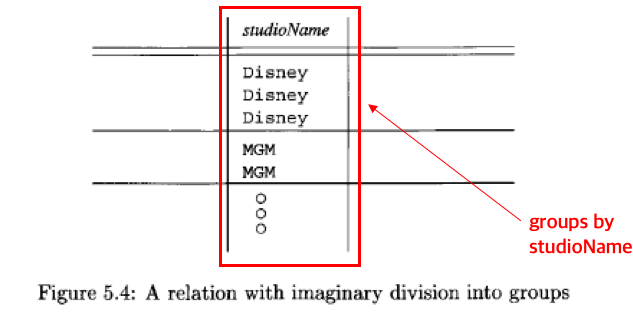
\includegraphics[width=0.7\linewidth]{images/worksheet_4_solution_1.png}
            \end{center}

        \end{itemize}

        \item $[(0, 1.5), (2, 4.5), (3,4)]$
        \item $[(0,1),(0,1),(2,3),(2,4),(3,4)]$
        \item $\gamma_{A, MAX(C)}([(2,3,4),(2,3,4)]) \to [(2,4)]$
        \item $[(0,1,\bot),(2,3,4), (2,3,4),(0,1,\bot),(2,4,\bot),(3,4,\bot)]$

        \bigskip

        \underline{\textbf{Notes:}}

        \bigskip

        \begin{itemize}
            \item $\accentset{\circ}{\bowtie}$ is an outerjoin operator
            \begin{itemize}
                \item $\accentset{\circ}{\bowtie}_L$ means Natural Left Outer Join
                \item $\accentset{\circ}{\bowtie}_R$ means Natural Right Outer Join
                \item $\accentset{\circ}{\bowtie}$ means Natural Full Outer Join
                \item $\bot$ means null
            \end{itemize}


            \item e.g. $U \accentset{\circ}{\bowtie} V$

            \bigskip

            \begin{center}
            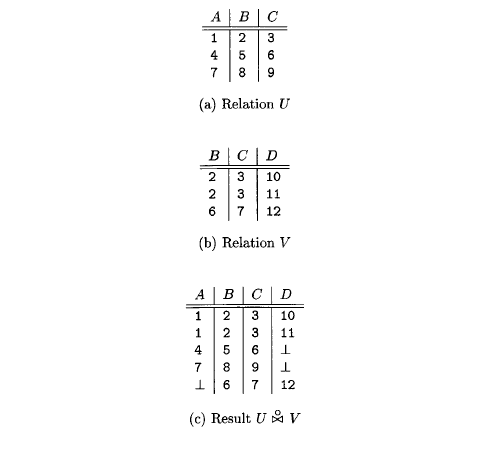
\includegraphics[width=0.7\linewidth]{images/worksheet_4_solution_2.png}
            \end{center}

        \end{itemize}

        \item $[(\bot,0,1),(\bot,2,4), (\bot,2,5),(2,3,4),(\bot,0,2),(2,3,4)]$
        \item $[(0,1,\bot),(2,3,4), (2,3,4),(0,1,\bot),(2,4,\bot),(3,4,\bot),\\
                (\bot,0,1),(\bot,2,4), (\bot,2,5),(2,3,4),(\bot,0,2),(2,3,4)]$

        \item

        $(0,1): \{(2,4),(2,5),(3,4),(3,4)\}$

        \bigskip


        But, $\{(2,3),(2,4),(3,4)\}$ from R and $\{(0,1),(0,2)\}$ in S dont match. So,

        \bigskip

        $[(0,1,2,4),(0,1,2,5),(0,1,3,4),(0,1,3,4),(0,1,2,4),(0,1,2,5),(0,1,3,4),(0,1,3,4),\\
         (2,3,\bot,\bot),(2,4,\bot,\bot),(3,4,\bot,\bot),(\bot,\bot,0,1),(\bot,\bot,0,2)]$

        \bigskip

        \underline{\textbf{Notes:}}

        \bigskip

        \begin{itemize}
            \item $R\accentset{\circ}{\bowtie}_CS$ is equivalent form of $\sigma_C({R \times S})$ but instead
            of filtering, the unmatching tuples filled with null.
        \end{itemize}
    \end{enumerate}

    \item

    \begin{enumerate}[a)]
        \item SELECT model FROM PC WHERE speed > 3.0;
        \item SELECT DISTINCT maker FROM Products NATURAL JOIN Laptops
        WHERE hd $>=$ 100;
        \item

        \begin{lstlisting}[language=SQL]
        SELECT model, price FROM (
            (SELECT model, price FROM PC NATURAL JOIN Products)
            UNION
            (SELECT model, price FROM Laptop NATURAL JOIN Products)
            UNION
            (SELECT model, price FROM Printer INNER JOIN Products ON Printer.model = Product.model)
        );
        \end{lstlisting}
        \item SELECT model FROM Printer WHERE color;
        \item

    \begin{lstlisting}[language=SQL]
    (SELECT DISTINCT makers FROM Products WHERE type='laptops') -
    (SELECT DISTINCT makers FROM Products WHERE type='pc');
    \end{lstlisting}

        \item

    \begin{lstlisting}[language=SQL]
    SELECT hd FROM PC WHERE EXISTS (
        SELECT hd, COUNT(model) FROM PC GROUP BY hd
        HAVING COUNT(model) > 2
    );
    \end{lstlisting}
    \end{enumerate}

    \item

    \begin{enumerate}[a)]
        \item SELECT class, country FROM classes WHERE bore $>=$ 16;
        \item SELECT * FROM Ships WHERE launched $<$ 1921;
        \item SELECT * FROM Outcomes WHERE result='sunk';
        \item SELECT * FROM Classes NATURAL JOIN Ships WHERE displacement $>$ 35000;
        \item
    \begin{lstlisting}[language=SQL]
    SELECT name, displacement, numGuns FROM Classes NATURAL JOIN (
        SELECT * FROM Ships INNER JOIN Outcomes ON Ships.name = Outcome.ship
    );
    \end{lstlisting}

    \item

    \begin{lstlisting}[language=SQL]
    (SELECT name FROM Ships)
    UNION
    (SELECT ship AS name FROM Outcomes);
    \end{lstlisting}

    \item

    \begin{lstlisting}[language=SQL]
    SELECT class, COUNT(class) FROM Ships
    GROUP BY Class
    HAVING COUNT(class) = 1;
    \end{lstlisting}

    \item

    \begin{lstlisting}[language=SQL]
    (SELECT countries FROM Classes WHERE type='bb')
    INTERSECT
    (SELECT countries FROM Classes WHERE type='bc');
    \end{lstlisting}

    \item

    Current attempt:

    \begin{lstlisting}[language=SQL]
    (SELECT Table1.name FROM Outcomes AS Table1 INNER JOIN Ships ON Outcomes.ship = Ships.name)
    \end{lstlisting}

    Took too much time. Omitted for now.

    \end{enumerate}

    \item

    \begin{enumerate}[a)]
        \item SELECT AVG(speed) FROM PC;
        \item SELECT AVG(speed) FROM Laptop HAVING price $>$ 1000;
        \item SELECT AVG(price) FROM PC NATURAL JOIN Product HAVING maker = 'A';
        \item

    \begin{lstlisting}[language=SQL]
    SELECT AVG(price) FROM (
        (SELECT model, price FROM PC NATURAL JOIN Product WHERE maker = 'D')
        UNION
        (SELECT model, price FROM Laptop NATURAL JOIN Product WHERE maker = 'D')
    );
    \end{lstlisting}
        \item SELECT speed, AVG(price) FROM PC GROUP BY speed;
        \item SELECT maker, AVG(screen) FROM Laptop NATURAL JOIN Product GROUP BY
        maker;
        \item

    \begin{lstlisting}[language=SQL]
    SELECT maker, COUNT(model) FROM Products GROUP BY maker HAVING
    COUNT(model) >= 3;
    \end{lstlisting}

        \item

    \begin{lstlisting}[language=SQL]
    SELECT maker, MAX(price) FROM PC
    NATURAL JOIN Products GROUP BY maker;
    \end{lstlisting}

        \item

    \begin{lstlisting}[language=SQL]
    SELECT speed, AVG(price) FROM PC GROUP BY speed
    HAVING speed > 2.0;
    \end{lstlisting}
    \end{enumerate}

    \item

    \begin{enumerate}[a)]
        \item SELECT COUNT(class) FROM Classes;

        \begin{mdframed}
            \underline{\textbf{Correct Solution:}}

            \bigskip

            SELECT COUNT(class) FROM Classes \color{red}HAVING type='bb'\color{black};
        \end{mdframed}
        \item SELECT class, AVG(numGuns) FROM Classes GROUP BY class;

        \begin{mdframed}
            \underline{\textbf{Correct Solution:}}

            \bigskip

            SELECT class, AVG(numGuns) FROM Classes GROUP BY class \\
            \color{red}HAVING type='bb'\color{black};
        \end{mdframed}

        \item SELECT AVG(numGuns) FROM Classes HAVING type='bb';
        \item SELECT class, MIN(launched) FROM Ships GROUP BY class;
        \item

    \begin{lstlisting}[language=SQL]
    SELECT class, COUNT(Ships.name) FROM Ships INNER JOIN Outcomes
    GROUP BY class ON Ships.name = Outcomes.ship
    HAVING result='sunk';
    \end{lstlisting}
    \end{enumerate}

    \item

    \begin{lstlisting}[language=SQL]
    SELECT name, MIN(movieYear) FROM MovieStar INNER JOIN StarsIn ON
    StarsIn.starName = MovieStar.name GROUP BY name HAVING COUNT(name) >= 3;
    \end{lstlisting}

    \item

    Yes. It is possible

    \begin{itemize}
        \item Rename aggregate columns using $\rho$
        \item Use $\sigma$ around $\rho(\gamma(\cdots))$
    \end{itemize}

    \item

    \begin{enumerate}[a)]
        \item

        INSERT INTO PC(model, speed, ram, hd, price)
        VALUES (1100, 3.2, 1024, 180, 2499);

        \bigskip

        INSERT INTO Product(maker, model, type)
        VALUES ('C', 1100, 'pc');

        \bigskip

        \underline{\textbf{Notes:}}

        \bigskip

        \begin{itemize}
            \item Insertion
            \begin{itemize}
                \item \textbf{Syntax:} INSERT INTO R($A_1,A_2,...,A_n$) VALUES ($v_1,...,v_n$)
                \item Inserts a tuple with values into relation R
                \item Values can be from select statement
            \end{itemize}

            \bigskip

    \begin{lstlisting}[language=SQL]
    \\ Example 1
    INSERT INTO StarsIn(movieTitle, movieYear, starName)
    VALUES('The Maltese Fiction', 1942, 'Sydney Greenstreet');

    \\ Example 2
    INSERT INTO Studio(name)
        SELECT DISTINCT studioName
        FROM Movies
        WHERE studioName NOT IN
            (SELECT name FROM Studio);
    \end{lstlisting}
        \end{itemize}

        \item

    \begin{lstlisting}[language=SQL]
    // SQL statement 1
    INSERT INTO Laptop(model, speed, ram, hd, screen, price)
        SELECT DISTINCT model + 110, speed, ram, hd, 17 AS screen, price + 500
        FROM PC;

    // SQL statement 2
    INSERT INTO Product(maker, model, type)
        SELECT DISTINCT maker, model + 110, 'laptop' AS type
        FROM Product WHERE type='pc';
    \end{lstlisting}

        \item

    \begin{lstlisting}[language=SQL]
    DELETE FROM PC
    WHERE hd < 100;
    \end{lstlisting}

        \bigskip

        \underline{\textbf{Notes:}}

        \bigskip

        \begin{itemize}
            \item Deletion
            \begin{itemize}
                \item \textbf{Syntax:} DELETE FROM $R$ WHERE $<\text{Condition}>$;

                \bigskip

                \underline{\textbf{Example:}}

                \bigskip

    \begin{lstlisting}[language=SQL]
    DELETE FROM StarsIn
    WHERE movieTitle = 'The Maltest Falcon' AND
          movieYeear = 1942 AND
          starName = 'Sydney Greenstreet';
    \end{lstlisting}
            \end{itemize}
        \end{itemize}

        \item

    \begin{lstlisting}[language=SQL]
    DELETE FROM Product
    WHERE maker = ALL(
        (SELECT maker FROM Product WHERE type='laptop')-
        (
            (SELECT maker FROM PRODUCT WHERE type='laptop')
            INTERSECT
            (SELECT maker FROM PRODUCT WHERE type='printer')
        )
    )
    \end{lstlisting}

        \item

    \begin{lstlisting}[language=SQL]
    UPDATE Product
    SET maker = 'A'
    WHERE maker = 'B';
    \end{lstlisting}

        \bigskip

        \underline{\textbf{Notes:}}

        \bigskip

        \begin{itemize}
            \item UPDATE
            \begin{itemize}
                \item \textbf{Syntax:} UPDATE $R$ SET $<\text{new-value assignments}>$ WHERE $<\text{condition}>$;
                \item updates tuples in database

                \bigskip

                \underline{\textbf{Example:}}

                \bigskip

    \begin{lstlisting}[language=SQL]
    UPDATE MovieExec
    SET name = 'Pres.' || name
    WHERE cert# IN (SELECT presC# FROM Studio);
    \end{lstlisting}

            \end{itemize}

        \end{itemize}

        \item UPDATE PC SET ram = 2 * ram, hd = 60 + hd;
        \item

    \begin{lstlisting}[language=SQL]
    UPDATE Laptop
    SET screen = screen + 1, price = price - 100
    WHERE model IN (
        SELECT model FROM Product
        WHERE type='laptop' AND
        maker = 'B'
    );
    \end{lstlisting}

    \end{enumerate}
\end{enumerate}

\end{document}